
%------------------------------------------------   
\section{Forecasting}
\label{sec:results-forecasting}

El forecasting permite realizar predicciones futuras basadas en un histórico de datos. Dado que el dataset \citep{dataset} contiene un histórico desde el año 2009, es idóneo para aplicar este tipo de técnicas. En esta sección se van a detallar los pasos necesarios para la aplicación del algoritmo de forecasting ARIMA \citep{arima}, realizando primero un preprocesamiento de los datos, seguido de la obtención de los conjuntos de datos para el entrenamiento y la validación del algoritmo. Por último, se aplicará el algoritmo ARIMA sobre 4 agrupaciones distintas de los datasets. \\

Todo esto se encuentra implementado en el notebook \code{src/forecasting.ipynb} \citep{master}.



%------------------------------------------------   
\subsection{Preprocesamiento}

Antes de poder aplicar el algoritmo de forecasting ARIMA \citep{arima}, el dataset debe ser preprocesado, al igual que se realizó con el clustering en la sección \ref{sec:clustering-preprocessing}. Sin embargo, no se ha realizado el mismo preprocesamiento. A continuación se detallan los pasos realizados en este preprocesamiento:

\begin{itemize}
 \item \textbf{Rellenar valores nulos}. En el dataset se han encontrado tres tipos de valores nulos: 
 \begin{itemize}
  \item \textbf{Valores de formato fecha}. Han sido rellenados con el valor \code{01/01/1990}.
  \item \textbf{Valores de formato texto}. Han sido rellenados con el valor de la cadena vacía.
  \item \textbf{Valores de formato texto asociados a identificadores}. Han sido rellenados con el valor \code{-1}.
 \end{itemize}
 
 \item \textbf{Eliminar de los registros} con valor distinto de \code{01/01/1990} en los campos \\ \code{DiscontinuedDate} y \code{ChemicalDateRemoved}, pues solo se precisan de aquellos registros de cosméticos que tengan productos químicos y no hayan sido retirados del mercado.

 \item \textbf{Agrupar por el campo} \code{InitialDateReported} sumando los valores del campo \\ \code{ChemicalCount}. Ya que el objetivo de la aplicación de forecasting es poder obtener una predicción de la cantidad de productos químicos que serán reportados en el futuro.
\end{itemize}

Tras aplicar este preprocesamiento nos queda un dataset con 1.863 registros y 2 características: \code{InitialDateReported} y \code{ChemicalCount}.




%------------------------------------------------   
\subsection{Obtención de los datasets de entrenamiento y validación}
\label{sec:dataset-validation}

Para poder realizar el forecasting, se necesita tener datos de entrenamiento y datos de validación (en adelante, \code{dataset} y \code{validation}, respectivamente). La obtención de estos datasets está ligada a que el dataset \citep{dataset} es incremental y se tienen almacenados las siguientes dos versiones del dataset, como se ha comentado en la sección \ref{sec:data-downloading}:

\begin{itemize}
 \item Carpeta \code{src/data/} \citep{master}, donde se almacena la versión más reciente del dataset.
 \item Carpeta \code{src/data\_backup/} \citep{master}, donde se almacena la versión anterior del dataset.
\end{itemize}

Con estas dos versiones, la obtención de los datasets \code{dataset} y \code{validation} se realiza de la siguiente manera: 

\begin{itemize}
 \item \code{dataset}. Contendrá todos los datos hasta los 5 meses previos al último mes de la versión \code{src/data\_backup/}. Es decir, suponiendo que el último mes de la versión \code{src/data\_backup/} es el 02/19 (Febrero del 2019), este dataset contendrá todos los datos antes del mes 09/18 (Septiembre del 2018): la última fecha de este dataset será el 31/08/2018 (31 de Agosto del 2018).
 \item \code{validation}. Contendrá el resto de datos. Es decir, siguiendo el mismo ejemplo, contendría los datos desde el 01/09/2018 (01 de Septiembre del 2018) hasta los datos de la última versión \code{src/data/}.
\end{itemize}

Así, se tiene un dataset de entrenamiento \code{dataset} con 1.749 registros y un dataset de validación \code{validation} con 114 registros.





%------------------------------------------------   
\subsection{Obtención de los parámetros \code{(p,d,q)}}

Al algoritmo de forecasting ARIMA \citep{arima} hay que proporcionarle tres parámetros \code{(p,d,q)} para el número de parámetros AR, las diferencias y los parámetros MA que definen el modelo. \\

Para saber cuáles son los valores de estos tres parámetros, se ha realizado una búsqueda ``en grid'' con cada uno de los siguientes valores:

\begin{itemize}
 \item \code{p}: desde 0 hasta 3.
 \item \code{d}: desde 0 hasta 2.
 \item \code{q}: desde 0 hasta 3.
\end{itemize}

teniendo así $4*3*4 = 48$ posibles modelos. La combinación \code{(p,d,q)} que dé el modelo ARIMA con menor error, será la combinación elegida para realizar el forecasting. El error se ha obtenido calculando la Error Cuadrático Medio \textit{(Root-Mean-Square Deviation (RMSE))} definido por la ecucación \ref{eq:rmse}, siendo $n$ el número total de observaciones, $T$ el conjunto de valores reales y $P$ el conjunto de valores predichos:

\begin{equation}
 RMSE = \sqrt{\frac{\sum\limits_{i=1}\limits^{n} (T_i - P_i) ^ 2}{n}}
\label{eq:rmse}
\end{equation}




%------------------------------------------------   
\subsection{Aplicación del algoritmo ARIMA}

Los datasets obtenidos en la sección \ref{sec:dataset-validation} contienen datos agrupados por días. Sin embargo, esto puede hacer que el modelo ARIMA sea muy complejo. Por lo que, para buscar el modelo que mejor se ajuste a los datos, se va a aplicar el modelo a las siguientes agrupaciones de los datasets:


%------------------------------------------------   
\subsubsection{Agrupando por mes}

Los datasets \code{dataset} y \code{validation} han sido agrupados por mes, de tal manera que los datasets se reducen a 110 y 6 registros, respectivamente. La Tabla \ref{tab:ts-grouping-by-month} muestra la configuración del modelo ARIMA aplicado a estos datasets, así como los RMSE obtenidos tanto en el entrenamiento como en la validación. La Figura \ref{fig:ts-grouping-by-month} muestra la comparativa de los valores reales con los predichos por el modelo.

\newpage
\begin{table}[!th]
\begin{tabular}{@{}ccc@{}}
\toprule
\code{(p,d,q)} & $RMSE_{dataset}$ & $RMSE_{validation}$ \\ \midrule
(1,1,0) & 18.822 & 15.212 \\
\bottomrule
\end{tabular}
\centering
\caption{Configuración y valores RMSE obtenidos por el modelo ARIMA agrupando por mes.}
\label{tab:ts-grouping-by-month}
\end{table}

\begin{figure}[!th]
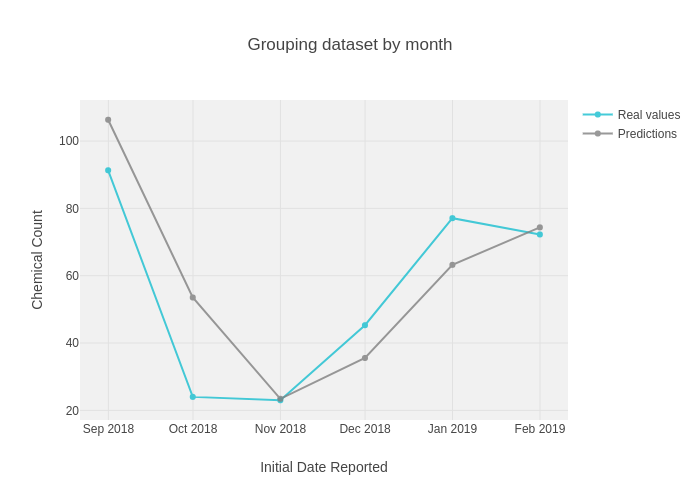
\includegraphics[scale=0.5]{figures/ts-grouping-by-month}
\centering
\caption{Comparación entre los valores reales y los predichos por el modelo ARIMA agrupando por mes.}
\label{fig:ts-grouping-by-month}
\end{figure}





%------------------------------------------------   
\subsubsection{Agrupando cada 15 días}

Los datasets \code{dataset} y \code{validation} han sido agrupados cada 15 días, de tal manera que los datasets se reducen a 223 y 12 registros, respectivamente. La Tabla \ref{tab:ts-grouping-by-15days} muestra la configuración del modelo ARIMA aplicado a estos datasets, así como los RMSE obtenidos tanto en el entrenamiento como en la validación. La Figura \ref{fig:ts-grouping-by-15days} muestra la comparativa de los valores reales con los predichos por el modelo.


\begin{table}[!th]
\begin{tabular}{@{}ccc@{}}
\toprule
\code{(p,d,q)} & $RMSE_{dataset}$ & $RMSE_{validation}$ \\ \midrule
(1,1,0) & 15.903 & 19.856 \\
\bottomrule
\end{tabular}
\centering
\caption{Configuración y valores RMSE obtenidos por el modelo ARIMA agrupando por cada 15 días.}
\label{tab:ts-grouping-by-15days}
\end{table}

\newpage
\begin{figure}[!th]
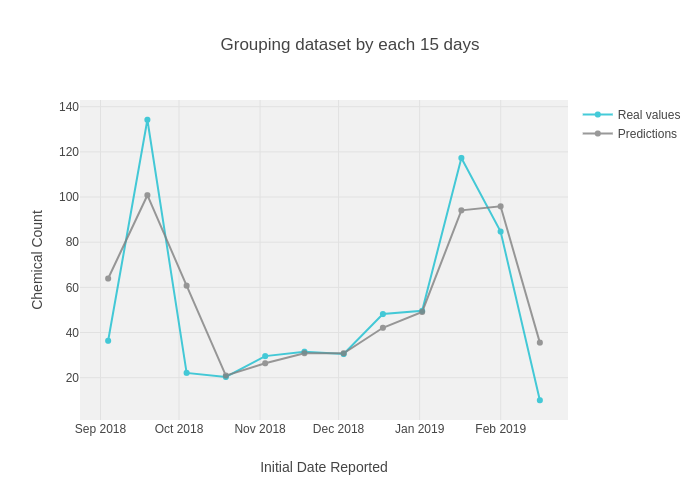
\includegraphics[scale=0.5]{figures/ts-grouping-by-15days}
\centering
\caption{Comparación entre los valores reales y los predichos por el modelo ARIMA agrupando por cada 15 días.}
\label{fig:ts-grouping-by-15days}
\end{figure}







%------------------------------------------------   
\subsubsection{Agrupando cada 7 días}

Los datasets \code{dataset} y \code{validation} han sido agrupados cada 7 días, de tal manera que los datasets se reducen a 467 y 25 registros, respectivamente. La Tabla \ref{tab:ts-grouping-by-7days} muestra la configuración del modelo ARIMA aplicado a estos datasets, así como los RMSE obtenidos tanto en el entrenamiento como en la validación. La Figura \ref{fig:ts-grouping-by-7days} muestra la comparativa de los valores reales con los predichos por el modelo.

\begin{table}[!th]
\begin{tabular}{@{}ccc@{}}
\toprule
\code{(p,d,q)} & $RMSE_{dataset}$ & $RMSE_{validation}$ \\ \midrule
(1,1,0) & 15.064 & 17.986 \\
\bottomrule
\end{tabular}
\centering
\caption{Configuración y valores RMSE obtenidos por el modelo ARIMA agrupando por cada 7 días.}
\label{tab:ts-grouping-by-7days}
\end{table}



%------------------------------------------------   
\subsubsection{Todo el dataset}

Los datasets \code{dataset} y \code{validation} no han sido agrupados, de tal manera que los datasets contienen 1.749 y 114 registros, respectivamente. La Tabla \ref{tab:ts-alldataset} muestra la configuración del modelo ARIMA aplicado a estos datasets, así como los RMSE obtenidos tanto en el entrenamiento como en la validación. La Figura \ref{fig:ts-alldataset} muestra la comparativa de los valores reales con los predichos por el modelo.

\begin{table}[!th]
\begin{tabular}{@{}ccc@{}}
\toprule
\code{(p,d,q)} & $RMSE_{dataset}$ & $RMSE_{validation}$ \\ \midrule
(1,1,0) & 12.905 & 23.571 \\
\bottomrule
\end{tabular}
\centering
\caption{Configuración y valores RMSE obtenidos por el modelo ARIMA sin agrupación.}
\label{tab:ts-alldataset}
\end{table}


\newpage
\begin{figure}[!th]
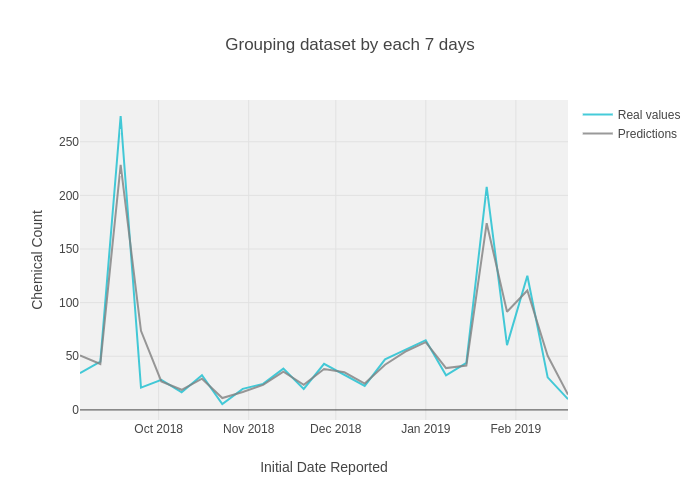
\includegraphics[scale=0.5]{figures/ts-grouping-by-7days}
\centering
\caption{Comparación entre los valores reales y los predichos por el modelo ARIMA agrupando por cada 7 días.}
\label{fig:ts-grouping-by-7days}
\end{figure}

\begin{figure}[!th]
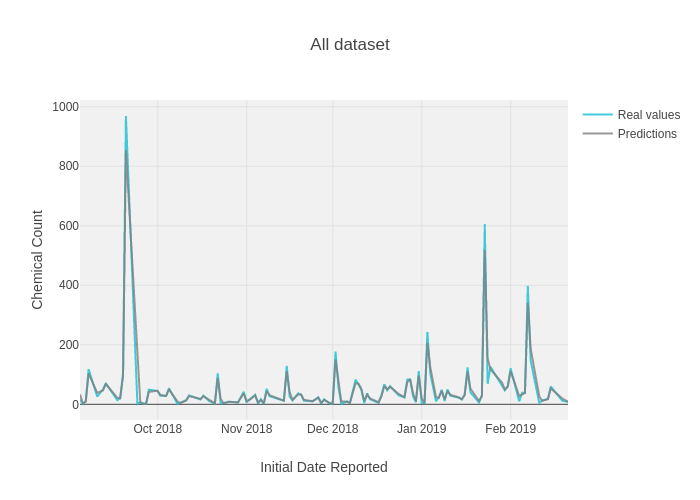
\includegraphics[scale=0.5]{figures/ts-alldataset}
\centering
\caption{Comparación entre los valores reales y los predichos por el modelo ARIMA sin agrupación.}
\label{fig:ts-alldataset}
\end{figure}
